% 作者:Yuchen Deng〔Zz〕 QQ群:19346666、111601117
% 欢迎加群共同维护与交流

\ifx\all\undefined
% 作者:Yuchen Deng〔Zz〕 QQ群:19346666、111601117
% 欢迎加群共同维护与交流

\documentclass[a4paper,fontset=fandol,zihao=-4,linespread=1.2]{ctexbook}

% \setCJKmainfont{FandolFang-Regular.otf} %中文字体
\setmainfont[Mapping=tex-text]{PT Mono} %英文字体
\ctexset{
  chapter/format = \Large\bfseries\centering,
  section/format = \large\bfseries,
  subsection/format = \normalsize\bfseries,
  chapter/beforeskip = 0pt,
  chapter/afterskip = 3ex plus 1ex minus 0.6ex,
  section/beforeskip = 2.5ex plus 1ex minus 0.5ex,
  section/afterskip = 1.5ex plus 1ex minus 0.3ex,
  subsection/beforeskip = 2ex plus 1ex minus 0.4ex,
  subsection/afterskip = 1ex plus 0.5ex minus 0.2ex,
  today = big
}

\usepackage{geometry} %布局
\ifx\publish\undefined
\geometry{left=2.3cm,right=2.3cm,top=2.0cm,bottom=2.0cm} %页边距
\else
\geometry{left=2.6cm,right=2.0cm,top=2.0cm,bottom=2.0cm} %页边距
\fi
\setlength{\parskip}{0.2\baselineskip} %段间距
\linespread{1.1} %行间距

\usepackage[unicode=false,colorlinks,linkcolor=blue]{hyperref} %超链接
\usepackage{silence} %屏蔽警告

\usepackage{tcolorbox} %盒子
\tcbset{colback=yellow!10, colframe=red!75!black}

\usepackage{listings} %代码框
\usepackage{xunicode} %代码框星号修复
\usepackage{xcolor} %颜色

\newfontfamily\mono{Source Code Pro}
\lstset{
	columns=flexible,
	numbers=left,
	numbersep=5pt,
	frame=shadowbox,
	xleftmargin=1em,
	xrightmargin=1em,
	backgroundcolor=\color{gray!2},
	rulesepcolor=\color{gray!50},
	basicstyle=\small\mono,
	keywordstyle=\color{blue!80},
	numberstyle=\tiny\mono\color{darkgray},
	commentstyle=\it\mono\color{gray},
	stringstyle=\color[RGB]{0,168,0},
	emphstyle=\color[RGB]{166,83,0},
	showstringspaces=false,
	breaklines=true,
	language=bash,
}

\makeatletter
\lst@CCPutMacro
    \lst@ProcessOther {"2D}{-{}}
    \@empty\z@\@empty
\makeatother


\title{\kaishu {\textcolor{blue!80}{Linux\hspace{0em}技术笔记 v1.0}} \footnote{\textcolor{red!80}{本笔记所涉及到的代码或命令需结合上下文说明并理解,不能简单地复制粘贴后在终端执行。}} \ldots}
\author{\fangsong Yuchen Deng〔语晨〕{\textcolor{red!80}{\hspace{0em}「QQ\hspace{0em}群\hspace{0.2em}19346666」}}\footnote{{\textcolor{blue!80}{\hspace{0em}Linux\hspace{0.3em}技术钻研群:19346666、111601117,拥抱开源,潜心钻研Linux技术!}}}}
\date{\kaishu\today}

\begin{document}
% 作者:Yuchen Deng〔Zz〕 QQ群:19346666、111601117
% 欢迎加群共同维护与交流

\maketitle
\pagenumbering{Roman}
\tableofcontents
\newpage
\pagenumbering{arabic}
\setcounter{page}{1}
\fi


\setcounter{chapter}{0}

\chapter{必须知道的知识}


\section{认识超级键}

\par 超级键(Super 键)也叫Windows键、徽标键或系统键,在现代的操作系统中通常用来呼叫出功能表或菜单。不同的桌面,该键或者与该键组合的快捷键功能略有不同,很多系统单独按下超级键时,会显示启动器(菜单),或者通过系统设置来让超级键显示启动器。启动器展示所有应用的入口,它的体验好坏、效率高低,自然非常重要。

\begin{figure} [htbp]
	\centering
	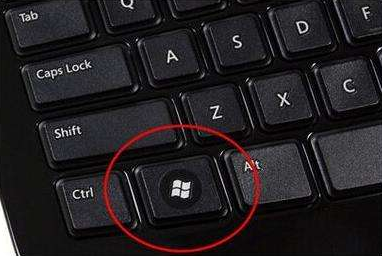
\includegraphics [scale=0.6] {images/ch01/2021-10-28_15-33-03.png}
	\caption{Super 键}
\end{figure}

\par 以下组合键建议你挨个尝试并熟练运用:
\begin{lstlisting}
    Super+S 切换工作区(多任务视图)
    Super+A 显示全部窗口
    Super+E 启动文件管理器
    Super+L 锁屏
\end{lstlisting}


\section{什么是终端}

\par Linux系统安装后,绝大多数的操作都是可视化的,用鼠标和键盘与桌面交互,就可以日常使用了。但为了更好的使用或者运维Linux系统,我们有时还是离不开命令行的。终端就是一个通过命令来与系统交互的窗口(应用),它的英文名字叫Terminal。像Ubuntu系统、KDE Plasma桌面,默认都绑定了“Ctrl+Alt+T”快捷键来启动终端,elementary OS 6则默认绑定“Super+T”快捷键。没有绑定快捷键的系统,如Debian、Fedora等,则可以通过启动器来启动,或者自定义快捷键启动。
\par 对GNOME桌面,默认的终端应用是gnome-terminal ,KDE Plasma桌面默认终端应用konsole,桌面不同,一般终端应用各异,但作用相同,用法类似。
\par 打开终端后,请依序执行以下\$之后的命令,你会有收获的。
\begin{lstlisting}
    $ help
    $ whatis man
    $ man man 1
\end{lstlisting}


\section{只在主目录工作}

\par 无论是通过快捷键“Super+E”,还是通过启动器运行“文件”或者“文件管理器”,默认展示的都是主目录内容。主目录也叫家目录、用户目录。
\par 请放弃寻找“C盘”、“D盘”之类的驱动器!文档、图片、视频、音乐、下载...都在主目录里,你工作、娱乐,都应该在主目录进行。如图\ref{fig:2021-10-28_22-31-38}所示。

\begin{figure} [htbp]
	\centering
	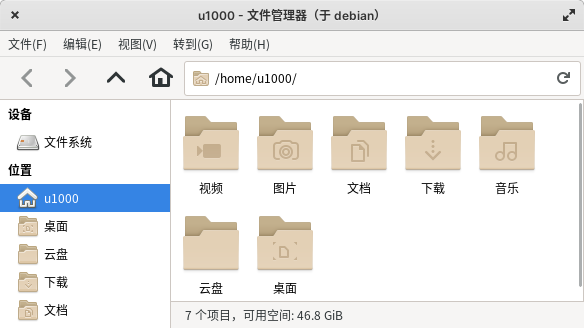
\includegraphics [width=0.8\textwidth]{images/ch01/2021-10-28_22-31-38.png}
	\caption{主目录}
	\label{fig:2021-10-28_22-31-38}
\end{figure}

\par 在终端里,主目录可以用符号“$\sim$”代替,现在请打开终端,运行下面的命令,看看输出并且与图片\ref{fig:2021-10-28_22-31-38}进行对比。
\begin{lstlisting}
    $ ls ~
    $ echo ~
    $ echo $HOME
    $ pwd
\end{lstlisting}

\par 如果你很好奇“pwd”的作用,正好可以在终端里执行“man pwd”练练手。
\par 回到文件管理器,按下“Super+H”快捷键,你会看到很多以“.”开头的目录和文件,它们默认是不显示的,即处在隐藏状态。再次执行“Super+H”会恢复隐藏。

\par 要在终端里显示隐藏文件,可以这样:
\begin{lstlisting}
    $ la
    $ ll
\end{lstlisting}

\par la和ll并不是新命令,而是ls添加适当参数的一个别名。终端执行:
\begin{lstlisting} [numbers=none]
    $ grep ls ~/.bashrc | grep ^alias
\end{lstlisting}
\par 输出:
\begin{lstlisting}
alias ll='ls -alF'
alias la='ls -A'
alias l='ls -CF'
\end{lstlisting}


\section{目录结构是棵树}

\par Linux目录结构就像是一棵倒挂的树,树干叫根目录,用符号“/”表示,一切从“根”开始,“/”是所有目录的起点。现在请在终端执行命令“ls /”,你会看到在根目录下,还有bin、boot、home、usr...等子目录。
\begin{lstlisting} [numbers=none]
    loaden@yuchen:~$ ls /
    bin   dev  home  lib32  libx32  mnt  proc  run   srv   sys  usr  vmlinuz
    boot  etc  lib   lib64  media   opt  root  sbin  swap  tmp  var
\end{lstlisting}

\par 每个目录或者文件都可以看作是树上的枝叶,目录就像树枝,文件就像树叶。树枝上还可以再长树枝,目录中也可以再嵌套目录,但树叶上就不可能再长出树枝了。
\par 在我当前正在使用的系统上执行下面的命令,输出如图\ref{fig:2021-10-31_16-05-54}所示的结果。

\begin{lstlisting} [numbers=none]
    $ tree / -L 4 --prune --matchdirs -P '文档|下载|*.docx'
\end{lstlisting}

\begin{figure} [htbp]
	\centering
	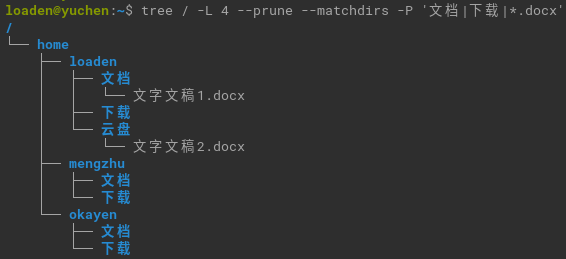
\includegraphics [width=0.8\textwidth]{images/ch01/2021-10-31_16-05-54.png}
	\caption{树状目录结构}
	\label{fig:2021-10-31_16-05-54}
\end{figure}

\par 我的用户名是loaden,严格的说,我的主目录只是loaden,它被建立在home目录下,对应的路径就是/home/loaden。依次类推,我妻子的主目录路径是/home/mengzhu,我儿子的主目录路径是/home/okayen。这条命令通过参数筛选了我想要的结果,请尝试不带参数直接执行“tree /”,可以加深理解。
\par 注意:/home不是家目录,而是所有用户主目录(家目录)的挂载点、父目录所在路径,它通常对应一个单独的分区。事实上Linux系统根目录下的各个子目录可以分布在不同的硬盘分区以及不同的硬盘设备上。
\par 大多数Linux目录结构都遵守FHS(Filesystem Hierarchy Standard)文件系统层次化标准。FHS定义了两层规范,第一层是“/”的各个子目录应该放什么文件数据,例如/etc应该存放设置文件,/bin应该存放可执行文件等。第二层则针对/usr及/var这两个目录的子目录来定义,例如/var/log存放日志、/usr/share存放共享数据等。


\section{为什么tree命令不存在}

\par 相信很多用户在执行前面讲述的tree命令时,会遇到这样的提示:
\begin{lstlisting} [numbers=none]
    Command 'tree' not found, but can be installed with:
    sudo apt install tree
\end{lstlisting}

\par 这是因为在很多Linux发行版上,tree这个软件包并没有默认安装。不同的发行版有不同的包管理工具,作用相同,用法类似。目前主流的软件包管理工具有三类,分别是Debian系的apt,红帽、Fedora系的dnf和Arch系的pacman。以安装tree软件包为例,我们只要打开终端,针对不同的发行版选择性的执行以下命令即可。
\begin{lstlisting} [numbers=none]
    $ sudo apt install tree
    $ sudo dnf install tree
    $ sudo pacman -S tree
\end{lstlisting}

\par sudo全称为:super user do,顾名思义:干超级用户root才能干的事!所以sudo最常用的功能就是提升命令的执行权限。
\par 现在很多Linux发行版都提供了“软件”、“商店”或者“应用中心”这样的图形化安装工具,很多应用我们用鼠标操作就可以安装或者卸载了。

\section{\$和\#的区别}

\par 打开终端或者登录shell后,闪烁的光标左边部分,称之为提示符prompt,通常普通用户提示符是美元符号\$,超级用户root提示符是井号\#。该符号表示等待输入命令。
\par 注意执行下面命令后,提示符和用户名的变化:

\begin{lstlisting} [numbers=none]
    loaden@yuchen:~$ sudo -i
    root@yuchen:~# exit
\end{lstlisting}

\par 截止目前我们介绍的命令,前面都有一个美元符号\$,意思是用普通用户的身份来执行命令。原则上,我们要尽量避免当终端里显示井号\#提示符时执行命令,要永远记得:权力越大,责任越大!滥用权限会给系统带来破坏,也给初学者带来疑惑。
\par 后面的讲解,如果命令前面是井号\#,说明需要以管理员权限来执行,建议在命令前添加sudo,或者通过“sudo -i”切换到root用户来执行。


\ifx\all\undefined
\end{document}
\fi
